\documentclass[pdftex,12pt,a4paper]{report}
\usepackage{dbstmpl}
\usepackage{subfigure}
\usepackage[T1]{fontenc}

% Hier die eigenen Daten eintragen
\global\arbeit{Bachelor Thesis}
\global\titel{Label Extraction from Image via Deep Learning}
\global\bearbeiter{Johannes Reichle}
\global\matrikel{04797218}
\global\betreuer{Prof.\ Dr.\ Rainer Schmidt}
\global\aufgabensteller{Random Ltd.}
\global\abgabetermin{XX.XX.2022}
\global\ort{Munich}
\global\fach{Information Systems and Management}

\begin{document}

\deckblatt
\erklaerung

\begin{abstract}
    Here abstract for \the\arbeit.
\end{abstract}


\tableofcontents

\chapter{Introduction}\label{ch:intro}
\section{Motivation}
\ac{OCR} is the concept of extracting typed, handwritten or printed text
from an image.
Techniques for this concept have improved a lot due to the advances in the field of
\ac{DL}~\citep{zhao_improving_2020}.
When compared to traditional methods \ac{DL} improves automation, effectiveness and
generalization~\citep{chen_text_2021}.
\ac{DL} is a technology based on \acp{NN} where data is processed
in multiple layers to extract complex features to solve a given problem~\citep{shrestha_review_2019}.
\ac{DL} has only caught on in the recent years as the big computational cost has been met
by improvement in computer hardware as well as automatic feature
learning~\citep{ponti_everything_2017, chen_text_2021}.
Finding the right solution in the space of \ac{DL} and applying these new capabilities to
the use case of extracting information of labels is the focus of this thesis.
This is an interesting task as performance of \ac{OCR} systems in complex scenes is still
challenging~\citep{zhao_improving_2020}.
Such scenes entail natural scenes captured by a camera.
\ac{OCR} in these conditions is also known as \ac{STR}~\citep{chen_text_2021}.
Factors such as complex backgrounds, noise, perspective and variability in fonts, colors and sizes,
of scene texts complicate the process~\citep{hu_gtc_2020,chen_text_2021}.
Therefore, it is critical to specify possible factors for the underlying problem and to find
criteria for evaluating feasibility.

% FIXME: adjust for pipeline instead of model
\section{Problem description}\label{se:problem}
The basic problem of this thesis is finding a viable solution for the extraction of textual
information from images with equipment labels.
However, it is difficult to assess how well an approach performs before it has been implemented and
tested on the specific problem or dataset~\citep{arpteg_software_2018}.
Therefore, it is useful to propose several approaches that might solve the problem from
different angles and different properties.

The problem has to first be analyzed in depth in order to find viable approaches for the solution.
This includes defining requirements such as detecting alpha-numeric strings or suitability despite
inadequate image conditions~\citep{ghosh_visual_2017, hu_gtc_2020}.
These requirements define properties that an approach must have in order to be classified as viable.
Thus the reasearch and subsequent discussion of techniques from end-to-end \ac{OCR} to dividing the
process into text detection and text recognition is centered around the requirements which are
given by the problem.

Subsequent aspects such as implementation, training, deployment and maintenance of a solution in a
production environment shall not be performed within the scope of this thesis.
However, because these aspects may vary depending on the approach, it is important to consider them when
discussing the viability for solving the problem.

% FIXME: add following
only model selection activity~\citep{ashmore_assuring_2021}
set into context to MLC lifecycle: Data Management, Model Learning (Model Selection, Training,
Transfer Learning, Hyperparameter Selection), Model Verificatoin

\section{Methodology}\label{se:methodology}
The methodology of this thesis can be described as a literature review.
As such, the research question guiding the process is most crucial: Which state of the art \ac{DL}
approaches for \ac{OCR} are viable for the use case of extracting textual label data from
images.
The following section describes how relevant literature is identified, analyzed and synthesised.

\section{Expected results}
% FIXME: kürzen
% FIXME: weg von literature review -> problem with criteria, analysing and summarizing research,
%               find viable approaches and compare properties for 5
In addition to a deeper understanding of the problem and its detailed definition, the literature
review lays the foundation for finding the right approach for the extraction of textual
information from images with equipment labels through literature review.
In the subsequent analysis different approaches are highlighted for their theoretical fit as a solution.

In the following section the structure of this thesis is listed and each chapter's expected
result is detailed along with its benefits for the overall objective of producing an overview of
state of the art \ac{OCR} relevant for the problem described in Section~\ref{se:problem}.
comprehension of the following chapters is gathered.
% FIXME: grammar above
This includes general principles of \ac{DL} and by extension \ac{ML} but also of \ac{OCR}.\@
In Chapter~\ref{ch:problem} the problem from Section~\ref{se:problem} is addressed in more detail.
The result shall be a firm understanding of functional and non-functional requirements both on the
technical and the business process side.
% FIXME: add exclusion criteria
These requirements are the point of focus for the further examination of \ac{OCR} techniques.
After laying the foundation, in Chapter~\ref{ch:research} current research in regards to the
identified requirements is examined.
The resulting overview can be viewed as a basis for a decision when it comes implementing a practical
solution.
Therefore it enables the discussion in Chapter~\ref{ch:discussion}.
Here not only the results and the availability of a solution but also the methodology of this work
are assessed critically.
The conclusion is a summary of the results compared to the expected results detailed in this chapter
as well as an outlook for further research into the topic.

\cleardoublepage%
\chapter{Theoretical Foundation}\label{ch:theoretical}
This chapter succinctly describes principles which build the foundation for later chapters.
Only the most relevant topics are touched upon, necessary details are explained in later chapters.
The mathematics that makes the techniques possible is not explained in depths as it would otherwise
exceed the scope of this work.
Whenever possible heavy mathematical notation is omitted if it does not aid the understanding of the
reader.

\section{Machine Learning}
To grasp \ac{DL}, a solid understanding of \ac{ML} has to be developed
first~\citep{goodfellow_deep_2016}.
This is because \ac{DL} is a subfield of \ac{ML}~\citep{chauhan_review_2018}.
The most well known definition for \ac{ML} comes from~\cite{mitchell_machine_1997}:
`A computer program is said to learn from experience $E$ with respect to some class of tasks $T$
and performance measure $P$, improves with experience $E$'.

% XXX: explain difference: model - algorithm
The task that the \ac{MLS} learns to perform, can range from approximating a function
(e.g.\ regression --- $f:\R^n \rightarrow \R^l$, classification ---
$f:\R^n \rightarrow \{1,\ldots,k\}$) to obtaining a different representation for the data that
has beneficial properties for further processing but preserves as much information as possible
(e.g.\ PCA for compression)~\citep{goodfellow_deep_2016}.
Note that the learning itself is not the task but merely the process of improving on performing the
task~\citep{goodfellow_deep_2016}.
One of the most well known \ac{ML} algorithms is Linear Regression.
In the following the algorithm is used as an example for explaining \ac{ML} principles.
As the name implies, Linear Regression is used to predict a value $\hat{y}\in\R$ given the input vector
$\x\in\R^n$ which is made up of the features $x_i$.
The goal is to approximate the ground truth $y$.
Linear is derived from the underlying model shown in Equation~\ref{eq:linReg}:
\begin{equation}\label{eq:linReg}
    f(\x;\w,b) = \w^{T} \cdot \x + b = \sum_{i=1}^{n} w_i x_i + b = \hat{y}
\end{equation}
The scalar product of the weights $\w\in\R^n$ and \x\ is added to the bias term $b\in\R$.
Both $\w,b$ are parameters that are learned by the model in order to optimize the
approximation~\citep{goodfellow_deep_2016}.

The performance of a model measures how well the task can be completed.
Depending on the task of the \ac{MLS}, different quantitative measures are used.
The metric Mean Squared Error (see Equation~\ref{eq:mse}) can be used for Linear Regression.
\begin{equation}\label{eq:mse}
    MSE =\frac{1}{m}\norm{{(\hat{\textbf{y}} - \textbf{y})}}^2
        =\frac{1}{m}\sum_{i=1}^m {((\w^T \x^{(i)} + b) - \yti)}^2
\end{equation}
Here $m$ denotes the number of examples $\xti$ with the associated targets $\yti$, used to calculate
the error~\citep{geron_hands-machine_2017,goodfellow_deep_2016}.
The goal is to minimize the generalization error which measures the expected performance on
previously unseen input~\citep{geron_hands-machine_2017}.
For this the test set is used, once the model has been trained.
The test set is a part of the available data~\citep{geron_hands-machine_2017, goodfellow_deep_2016}.
The generalization error can be divided into three components.
The bias error arises from simplifying assumptions for the model, the variance error measures the
variation in the model outcome depending on the data used for training.
Both these errors are influenced by the model's capacity which is why the relationship between them
is call the Bias/Variance tradeoff.
Lastly the irreducible error stems from not having measured all data as well as the variation
in real data and cannot be
reduced~\citep{ashmore_assuring_2021, james_introduction_2013,geron_hands-machine_2017}.

The experience part of \ac{ML} depicts the process where the algorithm is `experiencing' the training
dataset $\Xt$ and is learning important properties of the dataset.
In general, there are two paradigms for training: supervised and
unsupervised~\citep{goodfellow_deep_2016}.
Linear Regression is an example for supervised learning, as the model is using the ground truth value
to learn approximating $\yti$\ for the associated input
$\xti$~\citep{alzubi_machine_2018,goodfellow_deep_2016}.
For unsupervised learning on the other hand the algorithm is not directed to predict a target
value but to learn properties about the data and to leverage them for representation tasks
like compressing or denoising the data~\citep{goodfellow_deep_2016,geron_hands-machine_2017}.
In most cases training can be described as an optimization problem, i.e.\ as minimizing a
function --- the so called objective or loss function $L$~\citep{goodfellow_deep_2016}.
The MSE introduced earlier can be used for Linear Regression (see Equation~\ref{eq:mseOpt}).
This objective function has properties which make it suitable for models which have linear
output~\citep{goodfellow_deep_2016}.
\begin{equation}\label{eq:mseOpt}
    \min_{\w,b} MSE(\w,b)
\end{equation}
Note that for minimization the MSE is a function of $\w,b$ and not of $\x$, in terms of
predicting a value the MSE is a function of $\x$ parametrized by $\w,b$ (see Equation~\ref{eq:mseOpt}).
In Equation~\ref{eq:linReg} \w,$b$ are parameters that have to be learned in order to minimize
the generalization error~\citep{james_introduction_2013,geron_hands-machine_2017}.
For other tasks such as binary classification, the metric (e.g. \fone) and the
objective function (binary cross entropy loss) are different~\citep{geron_hands-machine_2017,
ho_real-world-weight_2020}.
For optimization the \ac{GD} algorithm is prevalent, especially in the subfield of \ac{DL}.
As the name suggests, the gradient is used to iteratively update the parameters $\w,b$ to arrive
at a minimum of the objective function (see Equation~\ref{eq:gradDescW}
and~\ref{eq:gradDescb})~\citep{geron_hands-machine_2017}.
\begin{equation}\label{eq:gradDescW}
    \w'\leftarrow \w-\epsilon\cdot\nabla_{\w} MSE(\w,b) = \w-\frac{2\epsilon}{m}\Xt^T (\Xt\w+b-\y)
\end{equation}
\begin{equation}\label{eq:gradDescb}
    b'\leftarrow b-\epsilon\cdot\frac{\delta}{\delta b} MSE(\w,b) = b-\frac{2\epsilon}{m}(\Xt\w+b-\y)
\end{equation}

\begin{figure}
    \centering
    {\scriptsize%
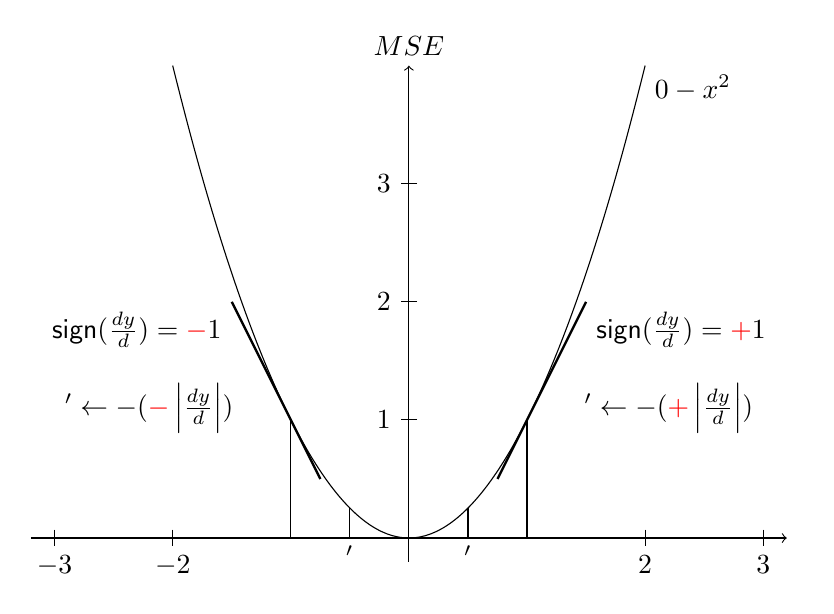
\begin{tikzpicture}[scale=1.5]
    \draw[->] (-3.2,0) -- (3.2,0) node[right] {$\w$};
    \draw[->] (0,-0.2) -- (0,4) node[above] {$MSE$};

    \foreach \x/\xtext in {2/2, 3/3}
        \draw[shift={(\x,0)}] (0pt,2pt) -- (0pt,-2pt) node[below] {$\xtext$};
    \foreach \x/\xtext in {-3/-3, -2/-2}
        \draw[shift={(\x,0)}] (0pt,2pt) -- (0pt,-2pt) node[below] {$\xtext$};
    \foreach \y/\ytext in {1/1, 2/2, 3/3}
        \draw[shift={(0,\y)}] (2pt,0pt) -- (-2pt,0pt) node[left] {$\ytext$};

    \draw (-2,4) parabola bend (0,0) (2,4) node[below right] {$\norm{0-x}^2$};
    \draw[-,line width=0.03cm] (0.75,0.5) -- (1.5,2) node[below right]
    {$\textsf{sign}(\frac{dy}{d\w})=\textcolor{red}{+}1$};
    \draw[-,line width=0.03cm] (-0.75,0.5) -- (-1.5,2) node[below left]
    {$\textsf{sign}(\frac{dy}{d\w})=\textcolor{red}{-}1$};

    \node at (2.2, 1.1) {$\w' \leftarrow \w - (\textcolor{red}{+}\left|\frac{dy}{d\w}\right|)$};
    \node at (-2.2, 1.1) {$\w' \leftarrow \w - (\textcolor{red}{-}\left|\frac{dy}{d\w}\right|)$};

    \draw[-] (1,1) -- (1,0);
    \draw[-] (-1,1) -- (-1,0);
    \draw[-] (0.5,0.25) -- (0.5,0);
    \draw[-] (-0.5,0.25) -- (-0.5,0);

    \node at (1, -0.2) {$\w$};
    \node at (-1, -0.2) {$\w$};

    \node at (0.5, -0.155) {$\w'$};
    \node at (-0.5, -0.155) {$\w'$};
\end{tikzpicture}
}

    \caption{Gradient descent for 1-dimensional objective function\label{fig:grad-desc}}
\end{figure}
The learning rate constant $\epsilon$ can be adjusted to speed up or slow down the `steps' which
can have different effects on the convergence~\citep{goodfellow_deep_2016}.
There are more sophisticated variations of the \ac{GD} algorithm which are more suited for practical
application (e.g. RMSProp, Adam)~\citep{geron_hands-machine_2017}.
Note that the process minimizes the test error with the test set $\Xt$.
The effect on the generalization error depends on model capacity which is the space of functions
the model enables~\citep{goodfellow_deep_2016}.
Linear Regression has the capacity to fit data with a linear relationship between features and
ground truth.
If the underlying relationship is more complicated, the model can only underfit the data (model
bias)~\citep{goodfellow_deep_2016}.
Polynomial Regression has more capacity for example.
Say the real relationship between features and ground truth now actually is linear;
the Polynomial Regression model can overfit for statistical outliers in the test set which is why
in this case the model with the lower capacity can achieve a lower generalization
error~\citep{geron_hands-machine_2017}.
Therefore, it is important to improve the bias/variance tradeoff.
Aside from model selection, there are different techniques used to prevent overfitting (e.g.
Regularization)~\citep{goodfellow_deep_2016}.
\begin{figure}[h]
    \centering
    \subfigure[Linear Regression underfit\label{fig:lin-reg-under}]{%
        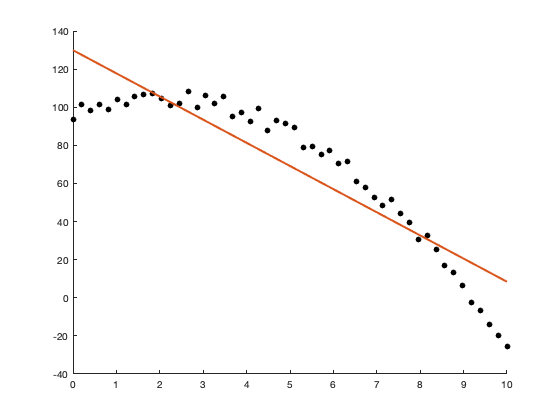
\includegraphics[width=0.45\textwidth]{img/Linear-Regression-underfit.png}
    }
    \subfigure[Polynomial Regression overfit\label{fig:pol-reg-over}]{%
        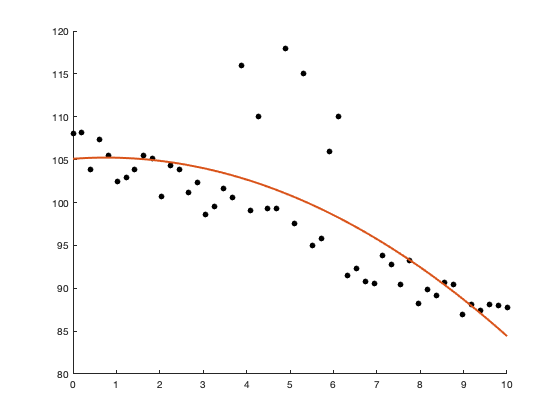
\includegraphics[width=0.45\textwidth]{img/Poly-Regression-overfit.png}
    }
    \caption{Regression with linear and polynomial model\label{fig:examples}}
\end{figure}

\section{Deep Learning}
In \ac{DL}, \acp{DNN} are leveraged to automatically learn new representations of data through
multiple layers of abstraction.
This makes \acp{DNN} powerful function approximators~\citep{goodfellow_deep_2016}.
In this section the basics of \acp{NN} are explained and popular basic architectures thereof are
introduced.

The most basic \ac{NN} is called a feedforward \ac{NN} or \ac{MLP} where the information only
flows in one direction (in contrast to \acp{RNN} or Transformers)~\citep{goodfellow_deep_2016}.
The network is made up of artificial neurons.
These neurons are arranged as a directed acyclic graph with multiple so
called layers~\citep{goodfellow_deep_2016}.
The first layer which receives the input features $\x$ is called the input layer, the last layer
which outputs the final estimation of $\hat{y}$ or $\hat{\y}$ is called the output layer, all layers in between
are called the hidden layers~\citep{shrestha_review_2019}.
The structure with which the \ac{NN} is build in terms of how many layers, how many neurons in each
layer and how they are connected, is called architecture~\citep{goodfellow_deep_2016}.
The number of layers $d$ is refered to as depths, whereas the dimensionality of those layers is
called the width $w$~\citep{goodfellow_deep_2016}.
\begin{figure}[ht]
	\centering
	\begin{tikzpicture}[shorten >=1pt]
		\tikzstyle{unit}=[draw,shape=circle,minimum size=1.15cm]
		\tikzstyle{hidden}=[draw,shape=circle,minimum size=1.15cm]

		\node[unit](x0) at (0,3.5){$x_0$};
		\node[unit](x1) at (0,2){$x_1$};
		\node at (0,1){\vdots};
		\node[unit](xd) at (0,0){$x_D$};

		\node[hidden](h10) at (3,4){$z_0^{(1)}$};
		\node[hidden](h11) at (3,2.5){$z_1^{(1)}$};
		\node at (3,1.5){\vdots};
		\node[hidden](h1m) at (3,-0.5){$z_{m^{(1)}}^{(1)}$};

		\node(h22) at (5,0){};
		\node(h21) at (5,2){};
		\node(h20) at (5,4){};

		\node(d3) at (6,0){$\ldots$};
		\node(d2) at (6,2){$\ldots$};
		\node(d1) at (6,4){$\ldots$};

		\node(hL12) at (7,0){};
		\node(hL11) at (7,2){};
		\node(hL10) at (7,4){};

		\node[hidden](hL0) at (9,4){$z_0^{(L)}$};
		\node[hidden](hL1) at (9,2.5){$z_1^{(L)}$};
		\node at (9,1.5){\vdots};
		\node[hidden](hLm) at (9,-0.5){$z_{m^{(L)}}^{(L)}$};

        \node[unit](y1) at (12,4){$\hat{y}_1^{(L+1)}$};
        \node[unit](y2) at (12,2.2){$\hat{y}_2^{(L+1)}$};
		\node at (12,1.2){\vdots};
        \node[unit](yc) at (12,0){$\hat{y}_C^{(L+1)}$};

		\draw[->] (x0) -- (h11);
		\draw[->] (x0) -- (h1m);

		\draw[->] (x1) -- (h11);
		\draw[->] (x1) -- (h1m);

		\draw[->] (xd) -- (h11);
		\draw[->] (xd) -- (h1m);

		\draw[->] (hL0) -- (y1);
		\draw[->] (hL0) -- (yc);
		\draw[->] (hL0) -- (y2);

		\draw[->] (hL1) -- (y1);
		\draw[->] (hL1) -- (yc);
		\draw[->] (hL1) -- (y2);

		\draw[->] (hLm) -- (y1);
		\draw[->] (hLm) -- (y2);
		\draw[->] (hLm) -- (yc);

		\draw[->,path fading=east] (h10) -- (h21);
		\draw[->,path fading=east] (h10) -- (h22);

		\draw[->,path fading=east] (h11) -- (h21);
		\draw[->,path fading=east] (h11) -- (h22);

		\draw[->,path fading=east] (h1m) -- (h21);
		\draw[->,path fading=east] (h1m) -- (h22);

		\draw[->,path fading=west] (hL10) -- (hL1);
		\draw[->,path fading=west] (hL11) -- (hL1);
		\draw[->,path fading=west] (hL12) -- (hL1);

		\draw[->,path fading=west] (hL10) -- (hLm);
		\draw[->,path fading=west] (hL11) -- (hLm);
		\draw[->,path fading=west] (hL12) -- (hLm);

		\draw [
            decorate,decoration={brace,amplitude=10pt},xshift=-4pt,yshift=0pt
        ] (-0.5,4) -- (0.75,4) node [black,midway,yshift=+0.6cm]{input layer};
		\draw [
            decorate,decoration={brace,amplitude=10pt},xshift=-4pt,yshift=0pt
        ] (2.5,4.5) -- (3.75,4.5) node [black,midway,yshift=+0.6cm]{$1^{\text{st}}$ hidden layer};
		\draw [
            decorate,decoration={brace,amplitude=10pt},xshift=-4pt,yshift=0pt
        ] (8.5,4.5) -- (9.75,4.5) node [black,midway,yshift=+0.6cm]{$L^{\text{th}}$ hidden layer};
		\draw [
            decorate,decoration={brace,amplitude=10pt},xshift=-4pt,yshift=0pt
        ] (11.5,4.7) -- (12.75,4.7) node [black,midway,yshift=+0.6cm]{output layer};
	\end{tikzpicture}
	\caption[Network graph for a MLP.]{
        Network graph of a $(L+1)$-layer perceptron with $D$ input units and $C$ output units.
        The $l^{\text{th}}$ hidden layer contains $m^{(l)}$ hidden units.
    }
	\label{fig:multilayer-perceptron}
\end{figure}

A neuron, the basic building block of \acp{NN}, receives input from neurons in the previous layer
and calculates a single value which is propagated to neurons in the following
layer~\citep{shrestha_review_2019}.
The value is calculated by feeding the received information into a Linear Regression model (see
Equation~\ref{eq:linReg}).
The resulting value is fed into an activation function $g$ which introduces nonlinearity, to allow
more complicated transformations of information and representation~\citep{goodfellow_deep_2016}.
\begin{equation}\label{eq:neuron}
    f(\x;\T) = g(\T\x)=\z
\end{equation}
Here $f$ denotes the function which is performed by a layer of neurons (linearity + activation).
The parameters of the individual neurons are grouped together to $\T$ ($\T_:,0$ equals 1 for the
bias term).
Popular activation functions include ReLU, sigmoid ($\sigma$) and softmax~\citep{shrestha_review_2019}.
\begin{equation}\label{eq:relu}
    ReLU(x)=\max(0,x)
\end{equation}
\begin{equation}\label{eq:sigmoid}
    \sigma(x)=\frac{1}{1+\exp(-x)}
\end{equation}
\begin{equation}\label{eq:softmax}
    {softmax(\x)}_i = \frac{\exp(x_i)}{\sum_j \exp(x_j)}
\end{equation}
While ReLU is the prevalent function for hidden layers, sigmoid (softmax) activation functions,
used for the output layer, are used to generate a bernoulli (multinouli) distribution which is
useful for classification tasks~\citep{goodfellow_deep_2016}.
\begin{comment}
\begin{figure}[ht]
    \centering
    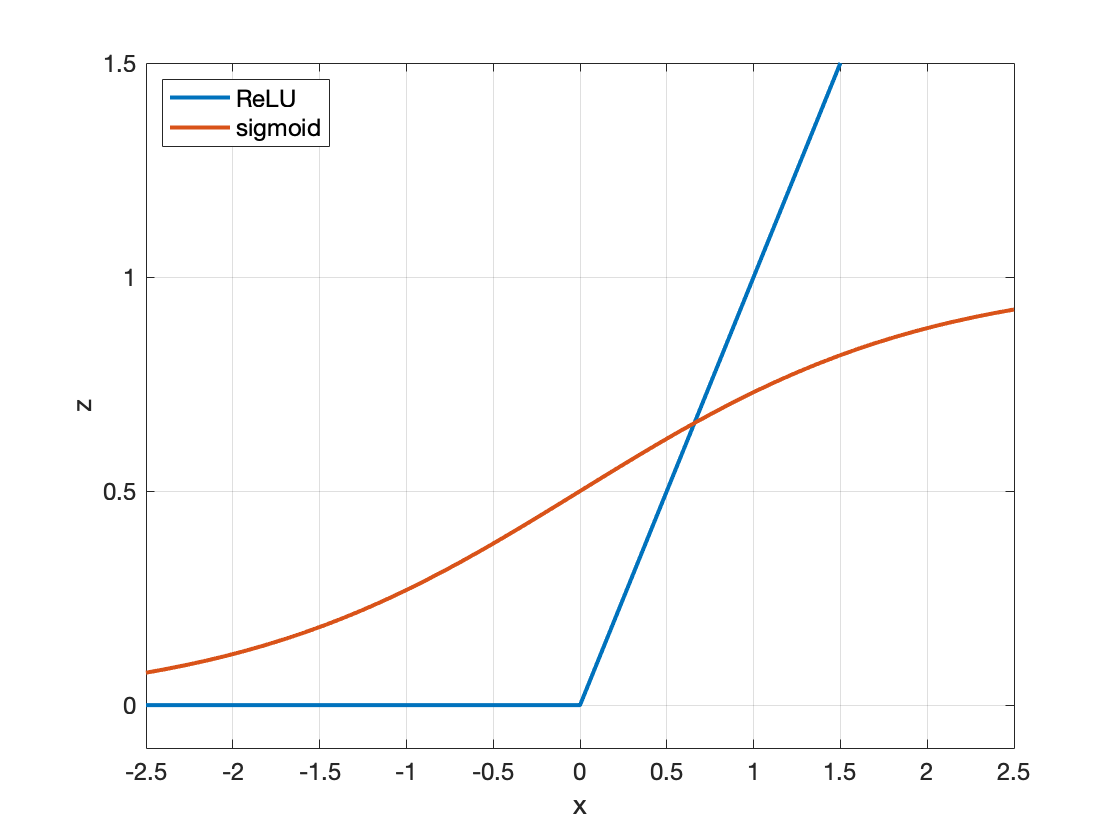
\includegraphics[width=0.6\textwidth]{img/activation-functions.png}
    \caption{Popular activation functions\label{fig:activation-functions}}
\end{figure}
\end{comment}
Note that for e.g.\ regression, the output layer can omit the activation
function~\citep{goodfellow_deep_2016}.
The calculation of the prediction is basically a concatenation of the functions defined by the
layers and their neurons, the process of which is called
forwardpropagation~\citep{ponti_everything_2017,goodfellow_deep_2016}.
\begin{equation}\label{eq:NNconcat}
    \hat{y}=f(\ldots f(f(\x;\T^{(1)});\T^{(2)})\ldots;\T^{(d)})
\end{equation}
$\T^{(i)}$ in Equation~\ref{eq:NNconcat} stands for the parameters in layer i with $\T^{(i)}_{j,:}$
being the parameters the $j$-th neuron in that layer~\citep{goodfellow_deep_2016}.
The forwardpropagation can also be described by a computational graph (see
Figure~\ref{fig:multilayer-perceptron})~\citep{goodfellow_deep_2016}.

The term \ac{DNN} comes from adding many hidden layers to the \ac{NN}~\citep{shrestha_review_2019}.
This allows for a more complicated function and better developed features or representations that
are extracted from the input feature vector $\x$~\citep{oyedotun_deep_2015}.
The \ac{DNN} can be trained as a whole, thus making feature engineering redundant in contrast to
normal \ac{ML} algorithms~\citep{arpteg_software_2018}.
The training algorithm is called backpropagation.
The training error is calculated through the objective function and is propagated
in conjunction with the output of forwardpropagation on each neuron~\citep{goodfellow_deep_2016}.
For this the chain rule of calculus can be used to modularly, recursively propagate the
loss backwards to use \ac{GD} (see Figure~\ref{fig:error-backpropagation}).
% TODO: not a real computation graph, ok?
\begin{figure}[ht]
	\centering
    \begin{figure}[ht]
	\centering
	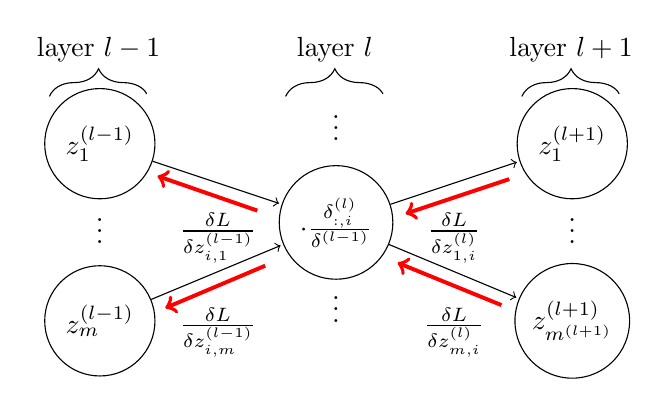
\begin{tikzpicture}[shorten >=1pt]
        \tikzstyle{unit}=[draw,shape=circle,minimum size =1.4cm]


		\draw [
            decorate,decoration={brace,amplitude=10pt},xshift=-4pt,yshift=0pt
        ] (-0.5,2.6) -- (0.75,2.6) node [black,midway,yshift=+0.6cm]{layer $l-1$};
        \node[unit](p1) at (0,2){$z_1^{(l-1)}$};
		\node at (0, 1){$\vdots$};
        \node[unit](pm) at (0,-0.25){$z_{m}^{(l-1)}$};

		\draw [
            decorate,decoration={brace,amplitude=10pt},xshift=-4pt,yshift=0pt
        ] (2.5,2.6) -- (3.75,2.6) node [black,midway,yshift=+0.6cm]{layer $l$};
		\node at (3, 2.3){$\vdots$};
        \node[unit](i) at (3,1){$\cdot\frac{\delta \z_{:,i}^{(l)}}{\delta \z^{(l-1)}}$};
		\node at (3, 0){$\vdots$};

		\draw [
            decorate,decoration={brace,amplitude=10pt},xshift=-4pt,yshift=0pt
        ] (5.5,2.6) -- (6.75,2.6) node [black,midway,yshift=+0.6cm]{layer $l+1$};
        \node[unit](k1) at (6,2){$z_1^{(l+1)}$};
		\node at (6, 1){$\vdots$};
		\node[unit](km) at (6,-0.25){$z_{m^{(l+1)}}^{(l+1)}$};

        \draw[->] (p1) -- (i);
        \draw[->] (pm) -- (i);

        \draw[->] (i) -- (k1);
		\draw[->] (i) -- (km);

        \node at (1.5,0.8){$\frac{\delta L}{\delta z_{i,1}^{(l-1)}}$};
        \node at (1.5,-0.4){$\frac{\delta L}{\delta z_{i,m}^{(l-1)}}$};

		\draw[->,red,line width=0.05cm] (2.1,0.45) -- (0.8,-0.1);
		\draw[->,red,line width=0.05cm] (2,1.15) -- (0.7,1.6);

        \node at (4.5,0.8){$\frac{\delta L}{\delta z_{1,i}^{(l)}}$};
        \node at (4.5,-0.4){$\frac{\delta L}{\delta z_{m,i}^{(l)}}$};

		\draw[->,red,line width=0.05cm] (5.1,-0.05) -- (3.75,0.5);
		\draw[->,red,line width=0.05cm] (5.2,1.55) -- (3.85,1.1);

    \end{tikzpicture}

	\caption[Backpropagation of errors through the network.]{
        Reverse traversing the network's computation graph,
        $\cdot \frac{\delta z_{:,i}^{(l)}}{\delta \w_i^{(l)}}$ is used for
        updating.\label{fig:error-backpropagation}
    }
\end{figure}

	\caption[Backpropagation of errors through the network.]{%
        Reverse traversing the network's computation graph,
        $\cdot \frac{\delta \z_{:,i}^{(l)}}{\delta \w_i^{(l)}}$ is used for
        updating the neurons parameters\label{fig:error-backpropagation}
    }
\end{figure}
The upstream gradient that is coming from neurons in the next layer is multiplied with the
jacobian matrix of the current neuron to produce the downstream gradient that is then used by
the preceding layer~\citep{boue_deep_2018,goodfellow_deep_2016}.
\begin{equation}\label{eq:backPropNeuronW}
    \frac{\delta L}{\delta\w} = \frac{\delta L}{\delta\z} \frac{\delta\z}{\delta\w}
\end{equation}
\begin{equation}\label{eq:backPropNeuronX}
    \frac{\delta L}{\delta\x} = \frac{\delta L}{\delta\z}\frac{\delta\z}{\delta\x}
\end{equation}
The result of Equation~\ref{eq:backPropNeuronW} is used to update the neuron's weights \w\ while
the result of Equation~\ref{eq:backPropNeuronX} is used for further propagation~\citep{boue_deep_2018}.
This calculation is performed until the first layer of the computational graph is
reached~\citep{goodfellow_deep_2016}.
Note that the algorithm can be performed with tensors of arbitrary
dimensionality~\citep{goodfellow_deep_2016}.

\section{Convoluational Neural Nets}
% basics
\acp{CNN} are a type of \ac{NN} that is also acyclic, like \acp{MLP}~\citep{chauhan_review_2018}.
It consists of a variety of components: fully connected layer, activation function,
convolutional layer, pooling layer~\citep{chauhan_review_2018,ponti_everything_2017}.
The fully connected layers combined with activation functions are the layers that make up
\acp{MLP}~\citep{ponti_everything_2017}.
% FIXME: 2d, 1d conv
% conv layer
A convolutional layer has multiple filters which consist of multiple kernels~\citep{chauhan_review_2018}.
For multi layer input, with $d$ so called channels, a filter has the same amount of kernels as there
are channels ($d$)~\citep{ponti_everything_2017}.
A kernel is a $n\times n$ square matrix made up of learnable parameters, so a filter is a tensor
$n\times n\times d$.
The convolution operation is the elementwise multiplication between the filter and overlapping
$n\times n$ subspace of the input (see Figure~\ref{fig:conv-layer})~\citep{ponti_everything_2017}.
\begin{figure}[ht]
    \centering
    \begin{tikzpicture}[scale=0.1]
	\matrix (mtr) [matrix of nodes,row sep=-\pgflinewidth, nodes={draw}]
	{
		0 & 1 & 1 & |[fill=red!30]| 1 & |[fill=red!30]| 0 & |[fill=red!30]| 0 & 0\\
		0 & 0 & 1 & |[fill=red!30]| 1 & |[fill=red!30]| 1 & |[fill=red!30]| 0 & 0\\
		0 & 0 & 0 & |[fill=red!30]| 1 & |[fill=red!30]| 1 & |[fill=red!30]| 1 & 0\\
		0 & 0 & 0 & 1 & 1 & 0 & 0\\
		0 & 0 & 1 & 1 & 0 & 0 & 0\\
		0 & 1 & 1 & 0 & 0 & 0 & 0\\
		1 & 1 & 0 & 0 & 0 & 0 & 0\\
	};

	\draw[very thick, red] (mtr-1-4.north west) rectangle (mtr-3-6.south east);

	\node [below= of mtr-5-4.south] (lm) {Input};

	\node[right = 0.2em of mtr] (str) {$*$};

	\matrix (K) [right=0.2em of str,matrix of nodes,row sep=-\pgflinewidth, nodes={draw, fill=blue!30}]
	{
		1 & 0 & 1 \\
		0 & 1 & 0 \\
		1 & 0 & 1 \\
	};
	\node [below = of K-3-2.south] (lk) {Kernel};

	\node [right = 0.2em of K] (eq) {$=$};

	\matrix (ret) [right=0.2em of eq,matrix of nodes,row sep=-\pgflinewidth, nodes={draw}]
	{
		1 & 4 & 3 & |[fill=green!30]| 4 & 1\\
		1 & 2 & 4 & 3 & 3\\
		1 & 2 & 3 & 4 & 1\\
		1 & 3 & 3 & 1 & 1\\
		3 & 3 & 1 & 1 & 0\\
	};
	\node [below = of ret-4-3.south] (lim) {Feature map};

	\draw[very thick, green] (ret-1-4.north west) rectangle (ret-1-4.south east);

	\draw[densely dotted, blue, thick] (mtr-1-4.north west) -- (K-1-1.north west);
	\draw[densely dotted, blue, thick] (mtr-3-4.south west) -- (K-3-1.south west);
	\draw[densely dotted, blue, thick] (mtr-1-6.north east) -- (K-1-3.north east);
	\draw[densely dotted, blue, thick] (mtr-3-6.south east) -- (K-3-3.south east);

	\draw[densely dotted, green, thick] (ret-1-4.north west) -- (K-1-1.north west);
	\draw[densely dotted, green, thick] (ret-1-4.south west) -- (K-3-1.south west);
	\draw[densely dotted, green, thick] (ret-1-4.north east) -- (K-1-3.north east);
	\draw[densely dotted, green, thick] (ret-1-4.south east) -- (K-3-3.south east);

	\matrix (K) [right=0.2em of str,matrix of nodes,row sep=-\pgflinewidth, nodes={draw, fill=blue!10}]
	{
		1 & 0 & 1 \\
		0 & 1 & 0 \\
		1 & 0 & 1 \\
	};

	\draw[very thick, blue] (K-1-1.north west) rectangle (K-3-3.south east);

	\node[anchor=south east, inner sep=0.01em, blue] at (mtr-1-4.south east) (xx) {\scalebox{.5}{$\times 1$}};
	\node[anchor=south east, inner sep=0.01em, blue] at (mtr-1-5.south east) (xx) {\scalebox{.5}{$\times 0$}};
	\node[anchor=south east, inner sep=0.01em, blue] at (mtr-1-6.south east) (xx) {\scalebox{.5}{$\times 1$}};
	\node[anchor=south east, inner sep=0.01em, blue] at (mtr-2-4.south east) (xx) {\scalebox{.5}{$\times 0$}};
	\node[anchor=south east, inner sep=0.01em, blue] at (mtr-2-5.south east) (xx) {\scalebox{.5}{$\times 1$}};
	\node[anchor=south east, inner sep=0.01em, blue] at (mtr-2-6.south east) (xx) {\scalebox{.5}{$\times 0$}};
	\node[anchor=south east, inner sep=0.01em, blue] at (mtr-3-4.south east) (xx) {\scalebox{.5}{$\times 1$}};
	\node[anchor=south east, inner sep=0.01em, blue] at (mtr-3-5.south east) (xx) {\scalebox{.5}{$\times 0$}};
	\node[anchor=south east, inner sep=0.01em, blue] at (mtr-3-6.south east) (xx) {\scalebox{.5}{$\times 1$}};

\end{tikzpicture}

    \caption{Convolution operation of a single kernel from a convolutional layer\label{fig:conv-layer}}
\end{figure}
The convolution operation is performed for every space in the input, spaces can be skipped if
stride is introduced~\citep{ponti_everything_2017}.
Often zero-padding is used to preserve the dimensions height and width between input and output of
the layer~\citep{ponti_everything_2017}.
The number of filters a convolutional layer applies is equal to the output channels that the layer
has which are often called feature maps~\citep{ponti_everything_2017}.
The result of a convolutional layer is usually fed into a activation function to introduce
nonlinearity like with fully connected layers.
The activation is performed on every element in the output und preserves the
dimensionality~\citep{ponti_everything_2017}.
% pooling
Pooling layers are used to reduce the spacial dimension (i.e.\ downsampling) of feature
maps~\citep{ponti_everything_2017}.
Pooling layers preserve the number of channels and have no learnable parameters. % FIXME: source
\begin{figure}[ht]
    \centering
    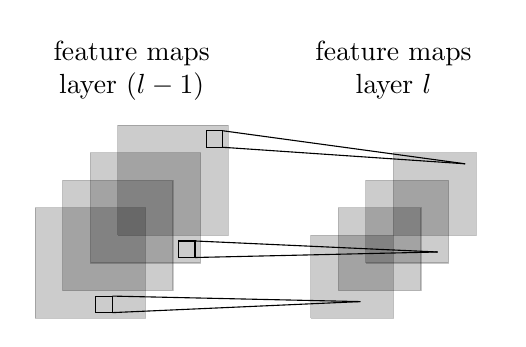
\begin{tikzpicture}[scale=0.7]
    \node at (1.75,4.5){\begin{tabular}{c}feature maps\\layer $(l-1)$\end{tabular}};

    \draw[fill=black,opacity=0.2,draw=black] (1.5,1.5) -- (3.5,1.5) -- (3.5,3.5) -- (1.5,3.5) -- (1.5,1.5);
    \draw[fill=black,opacity=0.2,draw=black] (1,1) -- (3,1) -- (3,3) -- (1,3) -- (1,1);
    \draw[fill=black,opacity=0.2,draw=black] (0.5,0.5) -- (2.5,0.5) -- (2.5,2.5) -- (0.5,2.5) -- (0.5,0.5);
    \draw[fill=black,opacity=0.2,draw=black] (0,0) -- (2,0) -- (2,2) -- (0,2) -- (0,0);

    \draw (3.1,3.1) -- (3.4,3.1) -- (3.4,3.4) -- (3.1,3.4) -- (3.1,3.1);
    \draw (2.6,1.1) -- (2.9,1.1) -- (2.9,1.4) -- (2.6,1.4) -- (2.6,1.1);
    \draw (1.1,0.1) -- (1.4,0.1) -- (1.4,0.4) -- (1.1,0.4) -- (1.1,0.1);

    \draw (3.4,3.4) -- (7.8,2.8);
    \draw (3.4,3.1) -- (7.8,2.8);

    \draw (2.9,1.4) -- (7.3,1.2);
    \draw (2.9,1.1) -- (7.3,1.2);

    \draw (1.4,0.4) -- (5.9,0.3);
    \draw (1.4,0.1) -- (5.9,0.3);

    \node at (6.5,4.5){\begin{tabular}{c}feature maps\\layer $l$\end{tabular}};

    \draw[fill=black,opacity=0.2,draw=black] (6.5,1.5) -- (8,1.5) -- (8,3) -- (6.5,3) -- (6.5,1.5);
    \draw[fill=black,opacity=0.2,draw=black] (6,1) -- (7.5,1) -- (7.5,2.5) -- (6,2.5) -- (6,1);
    \draw[fill=black,opacity=0.2,draw=black] (5.5,0.5) -- (7,0.5) -- (7,2) -- (5.5,2) -- (5.5,0.5);
    \draw[fill=black,opacity=0.2,draw=black] (5,0) -- (6.5,0) -- (6.5,1.5) -- (5,1.5) -- (5,0);
\end{tikzpicture}
%
    \caption{Pooling layer\label{fig:pool-layer}}
\end{figure}
Much like with convolutions, the pooling operation is slid across the height and weight dimensions
of the channels (possibly with stride) and the pooling operation is
performed~\citep{ponti_everything_2017,chauhan_review_2018}.
The most popular kind of pooling is maxpooling~\citep{ponti_everything_2017}.
For the operation only the maximum value of the current subspace of the current channel is
taken~\citep{chauhan_review_2018}.
\begin{figure}[ht]
    \centering
    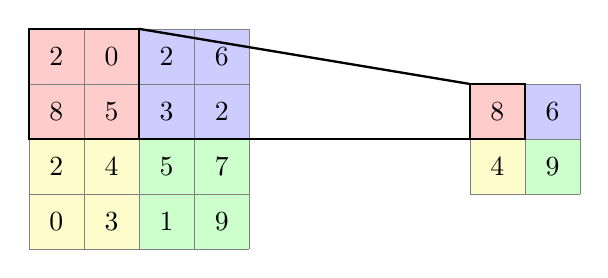
\begin{tikzpicture}[scale=0.7]
    \fill[yellow!20] (0,0) rectangle (2,2);
    \fill[red!20] (0,2) rectangle (2,4);
    \fill[green!20] (2,0) rectangle (4,2);
    \fill[blue!20] (2,2) rectangle (4,4);

    \draw[gray,very thin] (0,0) grid (4,4);

    \node at (0.5,0.5) {0};
    \node at (1.5,0.5) {3};
    \node at (0.5,1.5) {2};
    \node at (1.5,1.5) {4};

    \node at (2.5,0.5) {1};
    \node at (3.5,0.5) {9};
    \node at (2.5,1.5) {5};
    \node at (3.5,1.5) {7};

    \node at (0.5,2.5) {8};
    \node at (1.5,2.5) {5};
    \node at (0.5,3.5) {2};
    \node at (1.5,3.5) {0};

    \node at (2.5,2.5) {3};
    \node at (3.5,2.5) {2};
    \node at (2.5,3.5) {2};
    \node at (3.5,3.5) {6};

    \fill[yellow!20] (8,1) rectangle (9,2);
    \fill[red!20] (8,2) rectangle (9,3);
    \fill[green!20] (9,1) rectangle (10,2);
    \fill[blue!20] (9,2) rectangle (10,3);

    \draw[gray,very thin] (8,1) grid (10,3);

    \node at (8.5,1.5) {4};
    \node at (9.5,1.5) {9};
    \node at (8.5,2.5) {8};
    \node at (9.5,2.5) {6};

    \draw[draw=black, line width=0.3mm] (0,2) rectangle (2,4);
    \draw[draw=black, line width=0.3mm] (8,3) rectangle (9,2);

    \draw[-, line width=0.3mm] (2,4) -- (8,3);
    \draw[-, line width=0.3mm] (2,2) -- (8,2);

\end{tikzpicture}
%
    \caption{$2\times 2$ max pooling operation with stride 2\label{fig:pool-layer}}
\end{figure}
Popular \ac{CNN} architectures are explained in Chapter~\ref{ch:research}.

\section{Recurrent Neural Nets}

\begin{figure}[ht]
    \centering
    {\scriptsize%
\begin{tikzpicture}[%
    item/.style={circle,draw,align=center},
    itemc/.style={item,on chain,join},scale=0.5,
]

    \begin{scope}[start chain=going right,nodes=itemc,every
            join/.style={->},local bounding box=chain]
            \path node (At-1) {$\h^{(t-1)}$} node (At) {$\h^{(t)}$} node (At+1) {$\h^{(t+1)}$};
    \end{scope}

    \node[left=2em of chain,scale=1.5] (eq) {$\rightarrow$};

    \node[left=2em of eq,item] (AL) {$\h$};
    \path (AL.west) ++ (-1em,2em) coordinate (aux);
    \draw[->,rounded corners] (AL.east) -| ++ (1em,2em) -- (aux) |- (AL.west)
        node[left] (W) {};

    \draw[<-,dashed] (At-1) -- ++(-2,0);
    \draw[->] (At-1) -- (At)
        node[midway,above] (W) {};
    \draw[->] (At) -- (At+1)
        node[midway,above] (W) {};
    \draw[->,dashed] (At+1) -- ++(+2,0);

    \foreach \i in {t-1,t,t+1}
        {%
            \draw[->] (A\i.north) -- ++ (0,2em)
                node[above,item] (h\i) {$\hat{\y}_{\i}$};
            \draw[->] (A\i.north) -- ++ (0,2em)
                node[midway,right] (V\i) {};
            \draw[<-] (A\i.south) -- ++ (0,-2em)
                node[below,item] (x\i) {$\x_{\i}$};
            \draw[<-] (A\i.south) -- ++ (0,-2em)
                node[midway,right] (U\i) {};
        }

    \draw[white,line width=0.8ex] (AL.north) -- ++ (0,1.9em);
    \draw[->] (AL.north) -- ++ (0,2em) node[above,item] {$\hat{\y}$}
            node[midway,right] (V) {};
    \draw[<-] (AL.south) -- ++ (0,-2em) node[below,item,] {$\x$}
        node[midway,right] (U) {};

\end{tikzpicture}
}
%
    \caption{Recurrent neural net unroling\label{fig:rnn-unrolling}}
\end{figure}
RNN
\begin{itemize}
    \item LSTM:\ structure, rollout
    \item attention
\end{itemize}

\section{Transformers}
\begin{itemize}
    \item components: embedding (input \& output), positional encoding, multi-head attention,
        fully connected layer
    \item architecture: embedding \& positional encoding $\rightarrow$ encoder block
        $\rightarrow$ decoder block $\rightarrow$ softmax \& right shifting
\end{itemize}

\section{Scene Text Spotting}
%% intro
% def, ocr vs sts
\ac{OCR} is the concept of extracting typed, handwritten or printed text
from an image~\citep{zhao_improving_2020}.
Achieving satisfactory performance of \ac{OCR} systems in natural scenes is still
challenging~\citep{zhao_improving_2020, chen_text_2021}.
Such scenes entail natural scenes captured by a camera~\citep{chen_text_2021, baek_what_2019}.
The difficulties arise from diviersity and variability of text, complexity and interference from
backgrounds and imperfect imaging conditions.
In these conditions \ac{OCR} is known as \ac{STS}~\citep{long_scene_2021}.
% DL influence
Before the advent of \ac{DL}, researchers in the field had to hand-craft features~\citep{long_scene_2021}.
\ac{DL} automates the feature generation process with its representation and learning
capabilities~\citep{long_scene_2021,goodfellow_deep_2016}.
Because of this, \ac{DL} methods are the prefered tools for performing \ac{STS}~\citep{long_scene_2021}.
\ac{OCR} and \ac{STS} are often divided into two subcategories (Scene) Text Detection and (Scene)
Text Recognition~\citep{zhao_improving_2020, long_scene_2021,chen_text_2021}.
% STD, STR, end to end
For \ac{STD} the task is to localize text instances in the image, whereas the \ac{STR} task
is to recognize/categorize text from already cropped images~\citep{chen_text_2021}.
Note that a system which performs both \ac{STR} and \ac{STD} in one continuous pipeline are called
end-to-end approaches~\citep{chen_text_2021}.

%% evaluation metrics
% XXX: properties and pros for different metrics
% XXX: table with task, metric, properties/why it's used
To assess the performance of the developed approaches, the right evaluation metrics
have too be used.
% STD
The popular protocols Precision, Recall and the \fone\ are used for
comparison among approaches for \ac{STD}~\citep{long_scene_2021}.
The metrics are derived with values from the confusion matrix (see
Tabel~\ref{tb:confusionMatrix})~\citep{davis_relationship_2006}.
\begin{table}[ht]
    \centering\scriptsize
    \makebox[\textwidth][c]{\begin{tabular}{cccc}
        \toprule
                  & & \multicolumn{2}{c}{\textbf{Ground Truth}} \\
                  & & positive & negative \\
        \midrule
            \textbf{Prediction} & \multicolumn{1}{c|}{\makecell{positive\\negative}}
                            & \makecell{True Positive \\ False Negative }
                            & \makecell{False Positive \\ True Negative} \\
        \bottomrule
    \end{tabular}}
    \caption{Confusion Matrix\label{tb:confusionMatrix}}
\end{table}
\begin{equation}\label{eq:P}
    \text{Precision}=\frac{\text{True Positive}}{\text{True Positive + False Positive}}
\end{equation}
\begin{equation}\label{eq:R}
    \text{Recall}=\frac{\text{True Positive}}{\text{True Positive + False Negative}}
\end{equation}
\begin{equation}\label{eq:f1}
    F_1\text{-Score}=\frac{2\cdot \text{Precision}\cdot \text{Recall}}{\text{Precision}+\text{Recall}}
\end{equation}
The difference of metrics for the task manifests itself in the way the values of the confusion matrix
are calculated~\citep{long_scene_2021}.
Note that the tradeoff between False Positives and Fales Negatives manifests itself in the
Precision-versus-Recall curve~\citep{su_relationship_2015}.
\fone\ is also refered to as the harmonic mean (between Precision and Recall)~\citep{he_icpr2018_2018}.
% XXX: PvR curve figure
% XXX: introduce ROC curve --- ratio of true positive rate and false positive rate, and
%           relationship to PvR curve/AP
\ac{STD} differs mostly in the way the protocols match the prediction to the ground
truth~\citep{long_scene_2021}.
Detectors have multiple predictors which regress the placing and sizing of bounding boxes.
More information on this will follow in Chapter~\ref{ch:research}.
Matching is the process of assigning a bounding box prediction to the ground
truth, like in e.g.~\cite{liu_ssd_2016,liao_textboxes_2018}.
The PASCAL approach defines the \ac{IOU} (see Equation~\ref{eq:iou}).
\begin{equation}\label{eq:iou}
    \ac{IOU}=
            \frac{\text{area of intersection between truth and prediction}}{\text{area of union
            between truth and prediction}}
\end{equation}
For PASCAL, the prediction will be matched, if the \ac{IOU} value is larger than a
threshhold~\citep{long_scene_2021}.
A match is considered a True Positive, the other values are assigned accordingly~\citep{sun_icdar_2019}.
% more BB have IOU>threshhold -> depending on situation all or greatest value
Other evaluation approaches are mostly based on \ac{IOU}, e.g. MSRA-TD 500 evaluates the rotation
from the bounding box, compared to the truth in addition to the \ac{IOU}
threshhold~\citep{long_scene_2021}.
\cite{long_scene_2021} argues that researchers in the field of \ac{STD} should consider \ac{AP}
as the main evaluation protocol rather than \fone.
According to~\cite{su_relationship_2015}, \ac{AP} can be considered the area under the
Precision-versus-Recall curve.
\fone\ on the other hand only considers singular instances on that curve~\citep{long_scene_2021} and
is sensitive to the tradeoff while \ac{AP} is invariant to it~\citep{shi_icdar2017_2017}.
% STR
For \ac{STR} the evaluation can be based on character-level or word-level.
There is no need to match ground truth to prediction, as the image is already
cropped~\citep{long_scene_2021}.
The equations~\ref{eq:wordRecognitionAccuracy} and~\ref{eq:wordErrorRate} show metrics based on
word level~\citep{chen_text_2021}.
\begin{equation}\label{eq:wordRecognitionAccuracy}
\text{Word Recognition Accuracy} = \frac{\text{correctly recognized words}}{\text{total words}}
\end{equation}
\begin{equation}\label{eq:wordErrorRate}
    \text{Word Error Rate} = 1 - \text{Word Recognition Accuracy}
\end{equation}
An example for a character-based metric would be $1 - $NED where \ac{NED}
calculates the distance between prediction and ground truth (see Equation~\ref{eq:ned}).
\begin{equation}\label{eq:ned}
    \text{NED} = \frac{1}{N}\sum_{i=1}^N \frac{D(s_i,\hat{s}_i)}{\max(l_i,\hat{l_i})}
\end{equation}
D denotes the Levenshtein distance, s denotes the text, l denotes the text length and N is the total
number of text lines~\citep{shi_icdar2017_2017}.
For \ac{STR} \ac{NED} is used over the whole dataset~\citep{karatzas_icdar_2013}.
\ac{STS} is oriented to both \ac{STD} and \ac{STR}.
The prediction has to be matched to the ground truth like for \ac{STD}~\citep{long_scene_2021}.
For comparing predictions and matched the respective ground truths that have been matched, \ac{NED} is
used~\citep{chen_text_2021}.
For end-to-end recognition~\citep{karatzas_icdar_2013,karatzas_icdar_2015}, the main evaluation
protocols that are used include Precision, Recall, \fone\ and \ac{AED}~\citep{chen_text_2021}.
A sample is considered a True positive if the \ac{NED} distance between predictions and
matched ground truths is equal to 0~\citep{sun_icdar_2019} (on sample can have multiple text instances).
\ac{AED} is the sum of \ac{NED} values devided by the number of pictures~\citep{chen_text_2021}.
Note that competitions often define their own variants of the metrics,
e.g.~\cite{he_icpr2018_2018,shi_icdar2017_2017}.
Case sensitivity and matching criteria are examples for changing properties of metrics.

To compare approaches with these metrics benchmark datasets are used which have different
characteristics.
\begin{table}[ht]
    \centering\scriptsize
    \begin{tabular}{p{.25\textwidth}p{.05\textwidth}p{.05\textwidth}p{.15\textwidth}p{.25\textwidth}}
        \textbf{Dataset (year)}&\textbf{\ac{STD}}&\textbf{\ac{STR}}&\textbf{Text Orientation}
                                                            &\textbf{Characteristics} \\
        \toprule
        ICDAR (2013) & \checkmark& \checkmark&Horizontal& --- \\
        IIIT 5K-Word (2012) & &\checkmark&Horizontal& Cropped, variance in font, color, size and
                                                        noise~\citep{long_scene_2021} \\
        ICDAR (2015) & \checkmark& \checkmark&Multi-oriented& Low resolution, small text
                                                                instances~\citep{liao_mask_2020} \\
        MSRA-TD500 (2012) & \checkmark&&Multi-Oriented& Extreme aspect ratios~\citep{liao_mask_2020} \\
        ICDAR MLT (2017) & \checkmark&\checkmark&Curved& Multilingual~\citep{long_scene_2021}  \\
        SCUT CTW1500 (2017)& \checkmark& &Curved& --- \\
        Total-Text (2017) & \checkmark& \checkmark&Curved& --- \\
        \bottomrule
    \end{tabular}
    \caption{Benchmark datasets and their properties\label{tb:datasets}}
\end{table}
Table~\ref{tb:datasets} lists a couple of influencial benchmark datasets along with their key
properties.
ICDAR (2013) references the Focused Scene Text dataset~\citep{karatzas_icdar_2013} and ICDAR 2015
to the Incidental Text Competition dataset~\citep{karatzas_icdar_2015}.
The second and third column indicate whether the dataset provides annotations for the tasks.
The Text Orientation column specifies the most complicated orientation that is present in the dataset
(Curved $\subset$ Multi-oriented $\subset$ Horizontal).

\begin{figure}[h]
    \centering\scriptsize
    \subfigure[\scriptsize ICDAR (2013)~\citep{karatzas_icdar_2013}\label{fig:ICDAR-2013}]
        {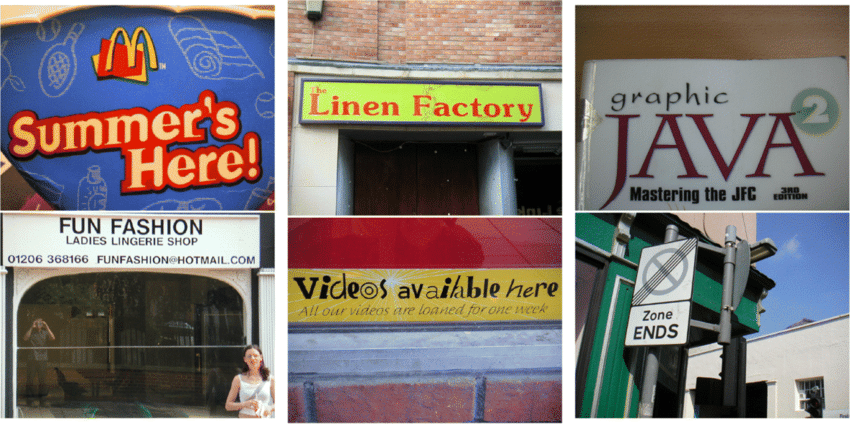
\includegraphics[width=0.30\textwidth]{img/Dataset-Examples/icdar-2013-examples.png}}
    \subfigure[\scriptsize ICDAR (2015)~\citep{karatzas_icdar_2015}\label{fig:ICDAR-2015}]
        {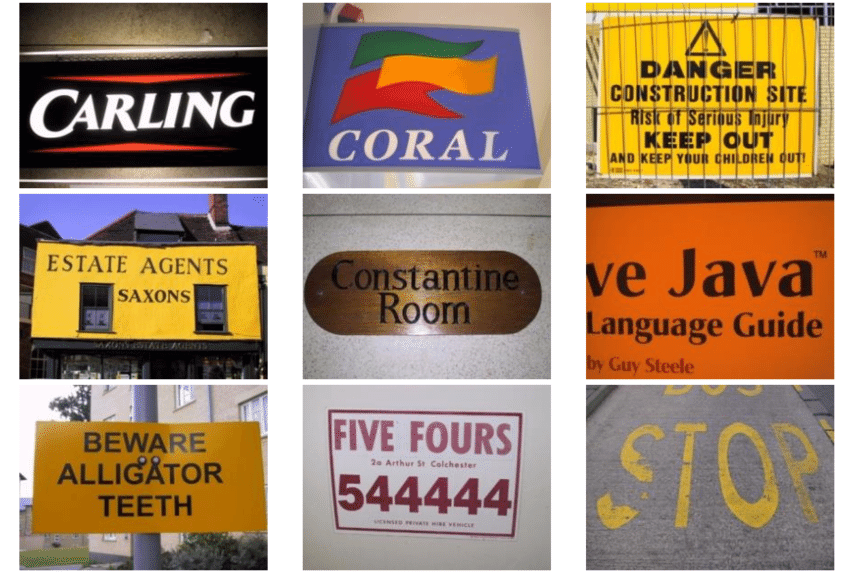
\includegraphics[width=0.30\textwidth]{img/Dataset-Examples/icdar-2015-examples.png}}
    \subfigure[\scriptsize ICDAR MLT (2017)~\citep{nayef_icdar2017_2017}\label{fig:ICDAR-2017}]
        {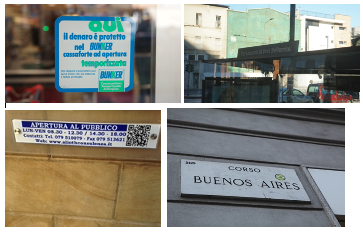
\includegraphics[width=0.30\textwidth]{img/Dataset-Examples/icdar-mlt-2017-examples.png}}
    \subfigure[\scriptsize IIIT 5k Word (2012)~\citep{mishra_scene_2012}\label{fig:IIIT-5k}]
        {
\includegraphics[width=0.30\textwidth]{img/Dataset-Examples/IIIT-5k-word-examples.png}}
    \subfigure[\scriptsize MSRA-TD500~\citep{cong_yao_detecting_2012}\label{fig:msra-td500}]
        {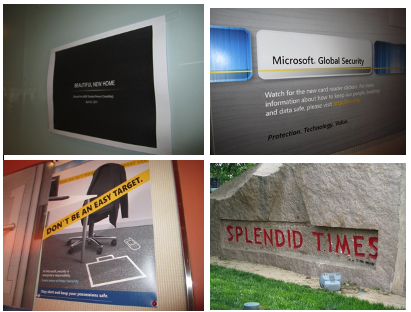
\includegraphics[width=0.30\textwidth]{img/Dataset-Examples/MSRA-TD500-examples.png}}
    \subfigure[\scriptsize Total Text (2017)~\citep{chan_total-text-dataset_2022}\label{fig:total-text}]
        {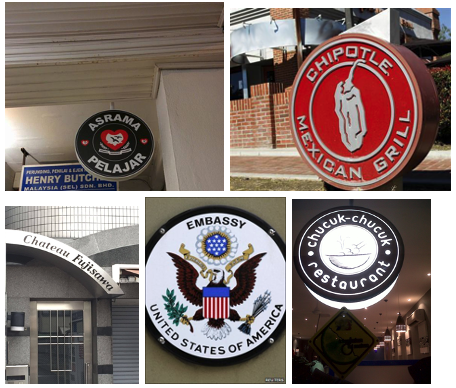
\includegraphics[width=0.30\textwidth]{img/Dataset-Examples/Total-Text-examples.png}}
    \subfigure[\scriptsize SCUT CTW1500 (2017)~\citep{yuliang_detecting_2017}\label{fig:SCUT-CWT1500}]
        {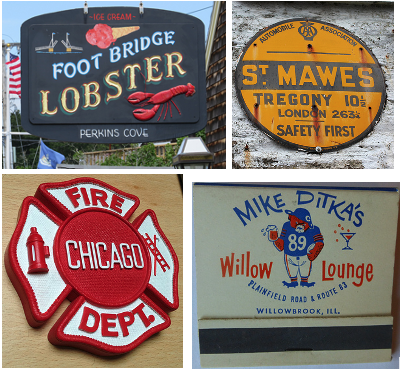
\includegraphics[width=0.30\textwidth]{img/Dataset-Examples/SCUT-CWT1500-examples.png}}
    \caption{Benchmark Data Set Examples\label{fig:dataset-examples}}
\end{figure}

\chapter{Problem analysis}\label{ch:problem}
This chapter entails an analysis of the problem which is the research question's foundation.
It is crucial, as the quality of requirements ultimately determines the quality of the overview and
subsequent analysis.
% FIXME: source for this?

Requirements for a software system that involves \ac{ML} and thus \ac{DL} differs from
the traditional approach. The data-driven software components are not entirely defined by the
programmer but are influenced by data.
The system acts with dependency on the test data~\citep{siebert_construction_2021}.
This poses a challenge in determining requirements and measuring quality of
results~\citep{nakamichi_requirements-driven_2020}.
Instead of categorizing functional and non-functional requirements, like for traditional
software projects~\citep{zowghi_requirements_2014}, qualities that a \ac{MLS} must possess
are defined.

\section{Use Case}
The problem can be depicted by a use case.
This use case sets the foundation for determining requirements for an
approach because qualities derive from the intended purpose of
use~\citep{siebert_construction_2021}.
Table~\ref{tb:useCaseQualities} gives an overview over the relevant properties that can be derived
from the use case.
\begin{table}[h]\label{tb:useCaseQualities}
    \centering\scriptsize
    \begin{tabular}{c l}
        \textbf{Offline Capabilities} & Perform extraction process offline \\
        \textbf{Alphanumeric recognition}    & Recognize alphanumeric strings such as serial \\
                                    & numbers \\
        \textbf{Semantics retention} & Retain semantics given implicitly be space, \\
                            & strucure and rotation of text in labels \\
    \end{tabular}
    \caption{Qualities specific to use case --- exclusion criterias}
\end{table}
For this thesis, the basic use case is as follows:
A technician takes a photo of a device label with his smart phone.
For this the technician is situated in locations like a cable shaft.
Due to this, there's no internet availability.
The process from taking the image to storing the extracted text safely must work offline.
The resulting image contains printed textual information which must be extraced by an application on
the smart phone.
Space and structure of this information can vary from label to label (see figure~\ref{fig:examples}).
The text, spacing and structure carries semantic information which can be important for later
processing in the scope of a business process~\citep{chen_text_2021}.
The goal is to extract the text and preserve semantics that are implicitly provided through
structure and space.
This means text and the respective coordinates, height, width and a possible rotation angle must
be output as the result~\citep{yang_learning_2021}.
Those values can then be transformed into other formats such as JSON or HTML as needed.
\begin{figure}[h]
    \centering
    \subfigure[Positive example\label{fig:good-example}]{\includegraphics[width=0.40\textwidth]
        {img/Image-Example-Positive.jpg}}
    \subfigure[Negative example\label{fig:bad-example}]{\includegraphics[width=0.40\textwidth]
        {img/Image-Example-Negative.jpg}}
    \caption{Examples for label images\label{fig:examples}}
\end{figure}
% XXX: use concept of representation for semantics retention
In addition to this, the labels can contain arbitrary alphanumeric strings such as serial numbers
(see figure~\ref{fig:examples}).
This results in the requirement that the \ac{DL} model has to be able to recognize sequences that
are not part of a predefined lexicon~\citep{ghosh_visual_2017}.
The qualities for the \ac{MLS} that can be derived directly from the use case (see
table~\ref{tb:useCaseQualities}) can be regarded as excluding criterias, because an approach
that does not possess the qualities in question, cannot be regarded as viable for the use case.

\section{Quality Identification}
In the article~\cite{ashmore_assuring_2021} the qualities are identified and assigned to different
challenges in regards to working with \ac{MLS}: Development Challenges, Production Challenges,
Organizational Challenges.
Because the only the Model Selection substage of the lifecycle is performed, the challenges and their
qualities are not relevant for this thesis, as they concern the operational aspect of \acp{MLS}.

% FIXME: make figure for system

In~\cite{nakamichi_requirements-driven_2020,siebert_construction_2021} systematic approaches for
identification and documentation of qualities are detailed.
In \acp{MLS} various entities interact to in order to produce the desired functionality.
The paper~\cite{nakamichi_requirements-driven_2020} suggests that in order to adequately evaluate
the qualities, it is essential to not only consider the model but the entire \ac{MLS}.
These entities are data, model, environment,
system/infrastructure~\citep{nakamichi_requirements-driven_2020, siebert_construction_2021}.
The article~\cite{siebert_construction_2021} differentiates between system and infrastrucure.
The infrastrucure represents given hardware and available libraries, whereas the system depicts
the software that surrounds the model in the runtime environment.
The data view pertains to the quality of development and runtime
data~\citep{siebert_construction_2021}.
% FIXME: better definition, there are cyclic architectures
The model consists of subcomponents organized in directed acyclc graph building a
pipeline.
This directed acyclic graph depicts everything from processing the images to the extracted
information~\citep{siebert_construction_2021}.
The environment entity covers the external aspects to the \ac{MLS} which may interact with
it~\citep{siebert_construction_2021}.
In the scope of this work the environment entails mostly the conditions in which images are taken.
For this thesis the entities data and system cannot be regarded as given.
The entities environment and infrastrucure are only losely defined through the use case.
That is why the systematic approaches cannot be performed in the scope of this thesis.
For example~\cite{siebert_construction_2021} proposes to follow the systematic CRISP-DM approach of
identifying qualities.
It cannot be performed due to the lack of data and the other entities.
Instead many qualities that are highlighted by research are taken into account along with critical
qualities (offline capabilities, alphanumeric recognition, semantic retention) that are directly
derived from the use case.
The Table~\ref{tb:LiteratureQualitiesModel} (p.~\pageref{tb:LiteratureQualitiesModel}) lists all
qualities that pertain to the model entity.
Different qualities are \textit{grouped together} for their similarities.
Because of their properties they can be evaluated jointly.
When it comes to documenting the identified qualities,
both~\cite{nakamichi_requirements-driven_2020} and~\cite{siebert_construction_2021} define a meta
model for qualities that combines qualities with
measurement methods and values and assignes them to an entity of the \ac{MLS}.
The implementation and testing phase are not performed in the scope of this thesis and the
difficulty in assessing the performance ahead of those phases, prevents the evaluation
of measurements.
Additionally, experimental results from literature can only be compared as long as factors such as
hardware, platform, source code, configuration and dataset are uniform~\citep{arpteg_software_2018}.
Comparing models through results of diferent papers is troublesome, because different papers
might use different evaluation and testing environments~\citep{baek_what_2019}.
This applies to studies that present an overview such as~\cite{chen_text_2021,long_scene_2021}.
These studies can only be regarded as guiding values because the performance for a specific dataset
cannot be predicted without testing on it~\cite{arpteg_software_2018}.
That's why targets for measurements are not defined, as evaluation would only deliver a false
sense of certainty.

\begin{table}[h]\label{tb:LiteratureQualitiesModel}
    \centering\scriptsize
    \begin{tabular}{p{.4\textwidth} p{.6\textwidth}}
        \textbf{Qualitiy} & \textbf{Source(s)} \\
        \toprule
        \textit{Appropriateness} \\
        Appropriateness &~\cite{siebert_construction_2021} \\
        Suitability &~\cite{siebert_construction_2021} \\
        Model Fitness --- Quality of Output Data &~\cite{nakamichi_requirements-driven_2020} \\
        \midrule
        \textit{Performance} \\
        Performance &~\cite{ashmore_assuring_2021,vogelsang_requirements_2019} \\
        Accuracy &~\cite{nakamichi_requirements-driven_2020} \\
        Model Fitness --- Degree of Correctness &~\cite{nakamichi_requirements-driven_2020,
                                                    zhang_machine_2020} \\
        Development correctness &~\cite{siebert_construction_2021} \\
        \midrule
        \textit{Robustness} \\
        Robustness &~\cite{ashmore_assuring_2021, hu_towards_2020, siebert_construction_2021} \\
        Robustness Against Change of Input Data &~\cite{nakamichi_requirements-driven_2020} \\
        Robustness Against Noise Data &~\cite{nakamichi_requirements-driven_2020} \\
        Relevance / bias-variance tradeoff &~\cite{siebert_construction_2021, zhang_machine_2020} \\
        Trained Model Generalization Performance Appropriateness
                                                    &~\cite{nakamichi_requirements-driven_2020} \\
        \midrule
        \textit{Reusability} &~\cite{ashmore_assuring_2021} \\
        \midrule
        \textit{Interpretability} \\
        Interpretability &~\cite{ashmore_assuring_2021, siebert_construction_2021, zhang_machine_2020}\\
        Understandability &~\cite{nakamichi_requirements-driven_2020} \\
        Transparency &~\cite{arpteg_software_2018} \\
        Model Explainability &~\cite{vogelsang_requirements_2019} \\
        Comprehensibility &~\cite{ashmore_assuring_2021} \\
        Comprehensiveness &~\cite{ashmore_assuring_2021} \\
        \midrule
        \textit{Fairness}\\
        Fairness &~\cite{siebert_construction_2021, zhang_machine_2020} \\
        Freedom from Discrimination &~\cite{vogelsang_requirements_2019} \\
        \midrule
        \textit{Performance Efficiency} \\
        Resource Utilization &~\cite{siebert_construction_2021,
                                nakamichi_requirements-driven_2020} \\
        Execution efficiency &~\cite{siebert_construction_2021} \\
        Temporal Performance &~\cite{nakamichi_requirements-driven_2020} \\
        \bottomrule
    \end{tabular}
    \caption{\ac{MLS} qualities identified for model entity through literature}
\end{table}
\FloatBarrier

\section{Quality Relevancy}
In addition to the qualities that arise directly from the use case, literature reveals a number of
common qualities in regards to \ac{MLS} (see Table~\ref{tb:condensedQualities}), some of which
can be regarded as relevant and other do not hold any relevance for the specific use case.
The qualities are taken from literature which covers \ac{ML} in general to literature
which covers scene text \ac{OCR}.
Only qualities that concern the model will be looked at, as the model is the focus of this thesis.
The qualities may however be influenced by other entities.

\begin{table}[h]\label{tb:condensedQualities}
    \centering\scriptsize
    \begin{tabular}{l l}
        \textbf{Relevant}                & \textbf{Irrelevant} \\
        Appropriateness         & Fairness  \\
        Performance             & Interpretability \\
        Robustness              & Reusability \\
        Performance efficiency  & \\
    \end{tabular}
    \caption{Condensed Qualities for model entity}
\end{table}

% Appropriateness
The appropriateness quality refers to the ability to perform the type of task that is required by
the use case~\citep{siebert_construction_2021,nakamichi_requirements-driven_2020}.
For this thesis this applies to scene text \ac{OCR} models.
Additionally, the properties which are derived from the use case (see Table~\ref{tb:useCaseQualities}),
can be grouped under this quality.

% Performance
`An ML model is performant if it operates as expected according to a measure (or set of measures)
that captures relevant characteristics of the model output'~\citep{ashmore_assuring_2021}.
For the performance quality, a measure is chosen depending on the type of task to be
solved~\citep{siebert_construction_2021}.
The F-Score is an example for a metric that is used to compare different
models~\cite{chen_text_2021, long_scene_2021}.
Performance is usually measured with a test dataset that is independent from training and validating
a model in order to approximate the generalization performance~\cite{goodfellow_deep_2016,
nakamichi_requirements-driven_2020}.

% Robustness
The robustness of a model concerns environmental uncertainty~\cite{ashmore_assuring_2021}.
Due to the uncontrolled environment in the practical aspect of taking the images on-site
beneficial image properties can not be guaranteed~\citep{chen_text_2021}.
Robust text extraction can be influenced by factors such as complex backgrounds, text form
(text rotation, font variability, arrangement), image noise (lighting conditions, blur,
interference and low resolution) and access (perspective, shape of
text)~\citep{oyedotun_deep_2015,ghosh_visual_2017,chen_text_2021}.
Therefore, these properties have to be accounted for when determining the viability for an approach.
Some of these factors do not change the expected prediction (noise), others do (text
form)\cite{hu_towards_2020}.
An example for bad image quality in regards to \ac{OCR} can be seen in figure~\ref{fig:bad-example}.
% FIXME: add \cite{long_scene_2021} difficulties

% Performance efficiency
Performance efficiency addresses time and resource utilization when the model is in use.
This does not involve the training phase but the execution or
prediction~\citep{siebert_construction_2021}.
The efficiency refers to low latency needs and to minimizing resource needs such as memory
usage or power consumption~\citep{nakamichi_requirements-driven_2020, siebert_construction_2021,
sourvanos_challenges_2018}.
This quality is especially important for usage on mobile devices in conjunction with
\ac{DNN}~\citep{sourvanos_challenges_2018, niu_26ms_2019}.
Note that performance efficiency is heaviliy influenced by the
infrastrucure~\citep{nakamichi_requirements-driven_2020, siebert_construction_2021}.
Because the efficiency needs fall mostly on the model, it is categorized as such and thus deemed
relevant in the scope of this thesis.

% Fairness
The first quality often found in research that is not relevant for the use case is fairness.
A fair model is free from discrimination bias.
For \ac{ML} this is can be a big problem, since discrimination can not only be influenced through
explicit programming in terms of the model but also through implicit knowledge from the
data~\citep{vogelsang_requirements_2019}.
For the use case however no relevance is attached.
The model can either recognize the text or it fails the task.

% Interpretability
The interpretability of a model helps to justify the output~\citep{ashmore_assuring_2021}.
The interpretability is twofold: explain what the model has learned, explain how a model given the
input comes to the output~\citep{vogelsang_requirements_2019}.
This can be challenging for two reasons.
\ac{ML} models used can be complex in terms of size and structure~\citep{ashmore_assuring_2021}.
Modular processing pipelines are continuously replaced with end-to-end
models which facilitates the tradeoff between interpretability and
performance~\cite{arpteg_software_2018}.

% Reusability
Another quality for a \ac{ML} model refers to how well a model intended for one task can be reused
for another related task.
% XXX: check whether trasnfer learning defined before
This can be beneficial because transfer learning can speed up the training, thus reducing training
cost~\citep{ashmore_assuring_2021}.
Reusability is not relavant in the scope of this work as it targets the training phase of the
\ac{ML} lifecycle.

\chapter{Current Research}\label{ch:research}
no transformers $\rightarrow$ self-attention mechanism is too computationally expensive???

model-pruning $\rightarrow$ remove connections for better performance
\section{Selection}


\section{Review}
`The great advances that have been made in fields such as computer vision and speech recognition,
have been accom- plished by replacing a modular processing pipeline with large neural networks
that are trained end-to-end [37]. In essence, transparency is traded for accuracy.
This is an unavoidable reality.'\citep{arpteg_software_2018}

include Pipeline differences

% FIXME: approaches to research: Faster R-CNN, Mask R-CNN, Yolo v3
% FIXME: look at Backbones: DETR-DC5-R101 and Faster RCNN-R101-FPN+

Two models that can be used in conjunction
\textbf{detection}~\citep{beom_text_2021}\\
uses RetinaNet structure~\citep{lin_focal_2018}\\
applies techniques from textboxes++~\citep{liao_textboxes_2018}

\textbf{character recognition}~\citep{beom_crnn_2021}\\
needs cropped text area as input\\
uses CRNN~\citep{shi_end--end_2015} $\rightarrow$ end-to-end learning, LSTM fir arbitrary length of
input and output, no need to apply detection and cropping to each single character

Open Source OCR engine~\citep{smith_overview_2007}
\begin{itemize}
    \item uses Deep Learning (found c++ code for layers in repo)
    \item Processing in step-by-step pipeline, some unusual stages\\
        1. Line and Word finding\\
        1.1. Line finding\\
        1.2. Baseline Fitting\\
        1.3. Fixed Pitch Detection and Chopping\\
        1.4. Proportional Word Finding\\
        2. Word Recognition\\
        2.1 Chopping Joined Characters\\
        2.2 Accociating Broken Characters\\
        3. Static Character Classifier\\
        3.1 Features\\
        3.2 Classification\\
        3.3 Training Data\\
        4. Linguistic Analysis\\
        5. Adaptive Classifier
\end{itemize}
Performs poorly with unstructured text with significant noise

An Efficient and Accurate Scene Text Detector~\citep{zhou_east_2017}

SOFT:\ Softmax-free Transformer with Linear Complexity~\citep{lu_soft_2021}

Generative Pretraining from Pixels~\citep{chen_generative_2021}
\begin{itemize}
    \item unsupervised representation learning (approach transfered from NLP)
    \item training of sequence Transformer to auto-regressively predict pixels without incorporating
        knowledge of 2D input structure
    \item Active part: GPT-2 scale model learns image representations and performs extremely well even
        when compared to supervised models
\end{itemize}

Learning High-Precision Bounding Box for Rotated Object Detection via Kullback-Leibler
Divergence~\citep{yang_learning_2021}
\begin{itemize}
    \item Deductive approach to rotated object detection
    \item box is `translated' to 2D-Gaussian $\rightarrow$ KLD with prediction and true gaussian as Loss
    \item LIMIT:\ cannot be directly applied to quadrilateral detection
\end{itemize}

DP-SSL:\ Towards Robust Semi-supervised Learning with A Few Labeled Samples~\citep{xu_dp-ssl_2021}
\begin{itemize}
    \item Semi-supervised learning:
        \begin{itemize}
            \item provides way to leverage unlabeled data by pseudo labels
            \item performs poorly and unstable when size of labeled data is very small (low quality
                of pseudo labels)
        \end{itemize}
    \item Data programming:
        \begin{itemize}
            \item paradigm for the programmatic creation of training sets
            \item existing methods rely on human experts to provide initial labeling functions (LF)
        \end{itemize}
    \item DP-SSL
        \begin{itemize}
            \item multiple-choice learning (MCL) based approach to automatically generate labeling functions
            \item scheme to generate probabilistic labels for unlabeled data
        \end{itemize}
\end{itemize}

which aspects to compare? quantitative, qualitative

\chapter{Discussion}\label{ch:discussion}
\section{Analysis}
Plan
\begin{itemize}
    \item Go down hierarchy and compare most important advances
\end{itemize}

For comparison: which Benchmark Dataset fits the problem the best?
\begin{itemize}
    \item~\cite{liao_mask_2020}:
        \begin{itemize}
            \item Rotated ICDAR 2013 (changed normal icdar): rotation robustness
            \item Total-Text: shape ropustness
            \item MSRA-TD500: aspect ratio ropustness
        \end{itemize}
    \item~\cite{yang_learning_2021}:commonly used for oriented text: ICDAR2015, ICDAR2017 MLT, MSRA-TD500
\end{itemize}

Important points:
\begin{itemize}
    \item ResNet is pretty much the Feature Extractor Benchmark
\end{itemize}

Recognition
\begin{itemize}
    \item Ability to cope with 2d text:
        CTC has problems,
        Attention/Encoder-Decoder based can be extended to work
    \item CTC prone to overfitting
    \item Attention has problems with long sequences
\end{itemize}

\section{Reflection}
Threats to validity!
\begin{itemize}
    \item~\cite{arpteg_software_2018}: different papers have different components
        $\rightarrow$ Hardware, Platform, Source Code, Configuration
        $\rightarrow$ studies can't really be compared
    \item~\cite{arpteg_software_2018}: `A major challenge in developing DL systems is the
        difficulties in estimating the results before a system has been trained and tested.'
    \item~\cite{long_scene_2021}: different interpretations of metrics (matching for \ac{STD},
        word/char for \ac{STR})
    \item~\cite{siebert_construction_2021,nakamichi_requirements-driven_2020}: all entities of
        \ac{MLS} should be inspected when developing a solution
    \item~\cite{baek_what_2019}: different papers use different evaluation and testing environments
    \item~\cite{baek_what_2019}: different papers use different subsets of the same dataset
        $\rightarrow$ discrepancies in performance
    \item~\cite{long_unrealtext_2020}: half of the widely adopted benchmark datasets have imperfect
        annotations $\rightarrow$ ignoring case-sensitivities and punctuations, and provide new
        annotations for those datasets
    \item~\cite{chen_text_2021}: inconsistency of datasets, priors and testing environments make
        comparison difficult
\end{itemize}

\section{Outlook}

\begin{itemize}
    \item next steps to practically solve problem $\rightarrow$  Data Collection, Data Cleaning,
        Data Labeling, Model Training, Model Evaluation, Model Deployment, Model
        Monitoring~\citep{watanabe_preliminary_2019}
    \item  Use Neural Architecture Search to automatically find right feature
        extractor~\citep{zhao_improving_2020}
    \item~\cite{siebert_construction_2021,nakamichi_requirements-driven_2020}: build system around
        model $\rightarrow$ e.g.\ supervision mechanism
    \item~\cite{shi_icdar2017_2017,he_icpr2018_2018}: adjust field to better metrics for evaluation
    \item~\cite{long_scene_2021}: general trend to move towards simpler,shorter pipeline
\end{itemize}

\chapter{Conclusion}
This thesis provides a comprehensive overview of techniques that are used for \ac{STS}.
The associated tasks and the different approaches help compare different
solutions for the identified qualified that are important for the use case
(appropriateness, performance/robustness, efficiency).

The overview and literature review reveal that \ac{STD} and \ac{STR} are concerned
with robust performance for multi-oriented and curved text instances.
For \ac{STD}, the more efficient \ac{BB} regression-based methods can detect multi-oriented text well.
Because of \acp{BB}' representational deficiencies, pixel-level segmentation-based methods are better for
detecting curved text.
However, they are more computationally expensive.
For the semantics retention subquality for appropriateness, it is, therefore, essential to consider
the text properties of the dataset.
The attention mechanism has become the primary approach for \ac{STR} robustness.
However, many innovations are concerned with the curved text rectification stage that both
\ac{CTC} and attention-based \ac{EnDe} solutions share.
\ac{CTC} has the advantage over the attention mechanism for recognition of alphanumeric strings
and efficiency, while attention is better with recognizing curved text.
For \ac{STS} research, 2-stage approaches are the focus because of their remarkable efficiency and
competitive performance.
The efficient combination of \ac{STD} and \ac{STR} stages and reuse of feature maps are topics
of the innovations in the field.

For future work, it would be helpful to consider different steps in the \ac{ML}
lifecycle~\citep{watanabe_preliminary_2019} or build a \ac{MLS} around the identified \ac{DL}
approach for \ac{STS}~\citep{siebert_construction_2021,nakamichi_requirements-driven_2020}.
An example would be to design a supervision mechanism for model monitoring that is important for
\ac{DL} in production systems~\cite{nakamichi_requirements-driven_2020,watanabe_preliminary_2019}.
Another possible step would be to design and carry out a comprehensive study to generate quantitative
data regarding the qualities that a \ac{STS} solution must possess.


\appendix

\chapter{References}

% Abbildungsverzeichnis (kann auch nach dem Inhaltsverzeichnis kommen)
\listoffigures

% delete group thing to have tables on new page
\begingroup
\let\clearpage\relax
% Tabellenverzeichnis (kann auch nach dem Inhaltsverzeichnis kommen)
\listoftables
\endgroup

% Literaturverzeichnis
%\bibliographystyle{dbstmpl}    % verwendet dbstmpl.bst
\bibliographystyle{alpha}

% alternative, vorinstallierte Stile sind z.B. plain oder abbrv
\bibliography{dbstmpl}         % verwendet dbstmpl.bib

\chapter{Code}
\end{document}
